N-Gram Graph is a NPL tool initially proposed by George Giannakopoulos\cite{Ngram} that use word or character n-gram in order to achieve documents summarization. The NGG tool basically slice the text in word or character n-gram and then represent them in a graph \emph{G = {N,E,L.W}} according the following structure:
\begin{itemize}
	\item N is the set of nodes created for every different n-gram in the text
	\item E represent the edge of the graph; where two node are connected by an edge if they are "near" according to a window-distance (if two n-gram appear in the same window they are near)
	\item L is a labelling function which give the label to every node and every edge (define the size of the n-gram)
	\item W is the weight function that gives weigh to every edge according to the number of times that two n-gram appear near one to the other
\end{itemize}

NGG so have the nice property to be language-neutral (make no assumption about the underlying language) and allow text manipulation trough graph operations.

In particular we used the \textbf{Intersection} operator between two graphs $G_1$ and $G_2$: which returns a resulting graph with only the common edges of $G_1$ and $G_2$ averaging the weights of the original edges assigned as the new edge weights. An example of this function is in figure \ref{fig:IntersectionOperation} where is computed the intersection between a graph $G_1$="aaabaab" and graph $G_2$="aabac" .

 
\begin{figure*}[htbp]
	\centering
			\begin{subfigure}[G1]
					{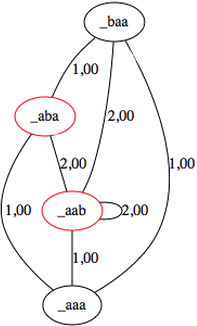
\includegraphics[width=6cm,height=7cm]{image/aaab.png}}	
			\end{subfigure}
			\begin{subfigure}[G2]
					{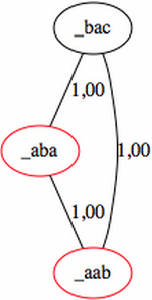
\includegraphics[width=4.5cm,height=7cm]{image/aac.png}}	
			\end{subfigure}
			\begin{subfigure}[Intersection Result]
					{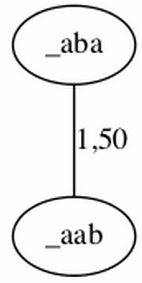
\includegraphics[width=3cm,height=6cm]{image/intersec-res.png}}	
			\end{subfigure}
			\caption[IntersectionOperation]{An example of the intersection operation}
	\label{fig:IntersectionOperation}
\end{figure*}


Combined to the Intersection operation with used a \textbf{Normalized Value Similarity}[NVS] function that for every n-gram rank, indicating how many of the edges contained in graph $G_i$ are also contained in graph $G_j$, considering also the weights of the matching edges and normalize the result respect the graph size. In particular $NVS(G_i,G_j) = \frac{VS(G_i,G_j)}{SS(G_i,G_j)}$ where:
\begin{equation}
 VS(G_i,G_j)=\frac{\sum e \in G_i \frac{\min(w_e^i, w_e^j)}{\max(w_e^i, w_e^j)}}{\max(\mid G_i \mid, \mid G_j \mid)}
\end{equation}

\begin{equation}
 SS(G_i,G_j)=\frac{\min(\mid G_i \mid, \mid G_j \mid)}{\max(\mid G_i \mid, \mid G_j \mid)}
\end{equation}

Since NGG tools allow to compute both the tweet-news correlation and summary creation, this methodology is split in different section.
\paragraph{Tweet-News Correlation}
To obtain a correlation between contradiction tweet and news, this methodology use the base idea of exploiting the NVS similarity function as a correlation function: higher the similarity of the tweets n-gram graph representation and the news n-gram representation, higher will be the correlation.

More in detail this procedure start reading all the contradiction tweet from the json file, concatenate the tweet text it in a unique string and compute the n-gram graph representation of the concatenated single. 

Due to the absence of memory lack problem, we prefer to decrease the computation time avoiding the usage of the scalable merging function proposed by George Giannakopoulos. The merging function based on a learning factor produce the same final result, but need a n-gram graph for every single tweet witch is more expensive in terms of computation time. It is strongly suggested to avoid the usage of intersection function over tweets, since tweet text contains many different language pattern determine a big chance to obtain an empty intersection graph (remember that intersection maintains only the common n-gram between the two document).

After computing the tweet graph, for every news is computed the NVS value between the tweet and news graphs. Since the NVS values have no time domain impact, a time windows is defined with the purpose of discharge from the correlation computation news that are distant in time. The correlation is computed only for news that were published in time slots defined by the contradiction point windows increased on both side by the time windows duration. The combined usage of a the truncating time windows  and the NVS similarity value produce the correlation value that we look for our first goal.
